\documentclass[12 pt]{article}
\usepackage{amsmath}
\usepackage{url}
\usepackage{graphicx}
\usepackage{setspace}
\usepackage{pgf}
\usepackage{tikz}
\usetikzlibrary{arrows,automata}
\usepackage[latin1]{inputenc}
\usepackage{verbatim}
\usepackage{lscape}
%\usepackage[margin=1.2in]{geometry}

	\addtolength{\oddsidemargin}{-.5in}
	\addtolength{\evensidemargin}{-.5in}
	\addtolength{\textwidth}{0.75in}
	\addtolength{\topmargin}{-1in}
	\addtolength{\textheight}{1.75in}
\begin{document}

\newcommand{\vocab}{\mathbf{v}}
\newcommand{\dtvec}{\mathbf{t}_\Delta}
\newcommand{\ctxvec}{\mathbf{t}_\text{ctx}}
\newcommand{\dt}{\Delta_t}


\section{Method}

Extract data collected from forums Timestamp, Author, Text Content. Using sliding window training method, group consecutive $w$ posts together and perform regression on $\Delta_t$. More formally, we are trying to learn a function $f$ such that $f(\mathbf{x}_{t-w},\hdots, \mathbf{x}_{t-1}) \approx \Delta_{t}$, where $\mathbf{x}_t$ is a post made at time $t$, and $\Delta_t$ is the time between the $t$-th post and the $(t-1)$-th post. The following are the features used:
\begin{description}
	\item[Previous time differences] All the time differences between posts made in the window. ($\mathbf{t}_\Delta$)
	\item[Time-based features] Day of week, Hour of day. Provides contextual information about when the post was made. ($\mathbf{t}_{\text{ctx}}$)
	
	\item[Content features (text)] Word frequency counts. Used regression to test effect of single regressor. Top $F$ features are selected for extraction. ($\mathbf{w}$)

\end{description}

\subsection{Evaluation metrics}
We use \emph{Mean Absolute Percentage Error} (MAPE), to measure the performance of the learnt model. This value does not reflect how well the model will do in a real-time setting, but gives an idea of how far off the model is given a window. This value is given by
\[
	\frac{1}{N}\sum^N_{i=1}\left|\frac{A_i-F_i}{A_i}\right|
\]

The \emph{$T$-score} metric measures the performance on a thread. This is the average time taken between a post being made and a visit made to retrieve that post. Limitations are that the value $T$-score does not factor in the number of times the page is hit. Keep track of the number of visits made as well. (Include explanation of $T$-score)

Viewing the posts made during the thread's lifetime as segmentations of the thread, and the visits made as hypotheses of where the segmentations are, we use the $Pr_{error}$ metric from Georgescul et. al. , 2006 as a measure of how close the predictions are to the actual posts.





\section{Results}

The results for experiments done with different combinations of the above specified features are shown in Table \ref{expt1}.
\begin{table}
	\footnotesize
	\begin{centering}
	\begin{tabular}{|l|c|c|c|c|c|c|c|c|}
	\hline
	\input{init_res}
	\hline
	\end{tabular}
	\caption{Experiment results}
	\label{expt1}
\end{centering}
\end{table}

Overall average and window average perform very poorly, on MAPE score, reflected in $T$-score.

Looking at $T$-score and no. of visits together, would seem that $\textbf{t}_\Delta$ is important feature (Including reduces $T$-score).

Using content (word frequency) features for prediction, gives only slight improvement.

High values for $Pr_{miss}$ and low for $Pr_{fa}$, are due to

	Mainly due to $Pr_{miss}$ being conditioned on the fact that there must be a segmentation/post there.
	Posts come in bursts, visits are fairly periodic, and intervals between visits are larger than post bursts.
	More posts than visits in places with posts, hence higher $Pr_{miss}$

	High no. of invalid predictions.
\begin{landscape}
\begin{figure}
	\centering
	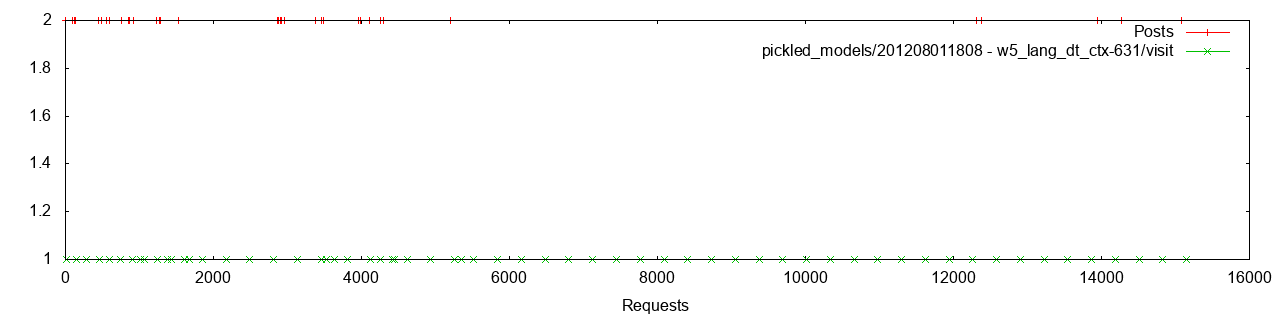
\includegraphics[scale=0.5]{example_seq.png}
	\caption{Visitation chart for a model using the $w=5, \mathbf{t}_\Delta, \mathbf{t}_{\text{ctx}},\mathbf{w}$ feature set. Invalid Predictions = 0.758, $Pr_{error} =  0.485$, $T$-score = 119.612, Posts = 41, Visits = 62}
\end{figure}
\end{landscape}

\begin{table}
	\footnotesize
	\begin{centering}
	\begin{tabular}{|l|c|c|c|c|c|c|c|c|}
	\hline
	\input{f_size}
	\hline
	\end{tabular}
	\caption{Experiment results: Varying feature sizes}
	\label{expt1}
\end{centering}
\end{table}


\bibliographystyle{acm}
\bibliography{report}
\end{document}
